%! TEX root = ../../master.tex
\lecture[Weghebungssatz. Lebesguelemma. Homotopieliftungssatz.]{Di 15 Jun 2021}{Hebungssätze}

\begin{theorem}[Weghebungssatz]\label{thm:weghebungssatz}
    Sei $p\colon E \to  X$ eine Überlagerung, und $w\colon  [0,1] \to  X$ ein Weg mit Anfangspunkt $x_0\coloneqq w(0)$. Sei $y\in p^{-1} (x_0)$ (also ein Punkt in der Faser von $x_0$). Dann existiert genau ein Weg $\tilde{w}\colon  [0,1] \to  E$, sodass $\tilde{w}(0) = y$ und $p \circ  \tilde{w} = w$, d.h. es kommutiert
    \[
    \begin{tikzcd}
        & E \ar{d}{p} \\
        I \ar[dashed]{ur}{\tilde{w}} \ar[swap]{r}{w} & X
    \end{tikzcd}
    \]
    Der Weg $\tilde{w}$ heißt \vocab[Weg!Hebung]{Hebung} oder \vocab[Weg!Lift]{Lift} von $w$.  
\end{theorem}

\begin{oral}[auf Nachfrage]
    Wir können uns den Endpunkt des Weges $\tilde{w}$, also $\tilde{w}(1)$, nicht aussuchen. Dieser ist aber eindeutig bestimmt durch die Wahl des Anfangspunktes $\tilde{w}(0) = y$.

    Wir wissen also, dass dieser Endpunkt existiert und eindeutig bestimmt ist, können aber noch keine Aussage darüber treffen.

    Zudem werden wir sehen, dass der Endpunkt nicht notwendigerweise der Anfangspunkt sein wird, selbst wenn es sich bei $w$ um eine Schleife handelt.
\end{oral}

\begin{proof}
    \underline{1. Fall}: Wir nehmen an, dass $p$ trivial ist, d.h. wir finden $F$, sodass kommutiert:
    \[
    \begin{tikzcd}
        E \ar{rr}{\cong}[swap]{u} \ar[swap]{dr}{p} & & X\times F \ar{dl}{\pr_X} \\
    & X
    \end{tikzcd}
    \]
    Wir müssen also zeigen, dass genau eine Hebung $\tilde{w}\colon I \to  X\times F$ existiert mit $\tilde{w}(0) = u(y)$. Sei $u(y) = (x_0,f)$ mit $f\in F$. Wir definieren nun
    \[
        \tilde{w}(t) = (w(t),f)
    .\] 
    d.h. wir heben den Weg einfach nach $X\times \left \{f\right\} \cong X$. Dann ist $\tilde{w}(0) = (w(0),f) = (x_0,f) = u(y)$, und die Projektion ist genau
    \[
        \pr_X(\tilde{w}(t)) = w(t)
    .\] 
    wie gewünscht.

    \underline{Eindeutigkeit}:  Sei $\tilde{\tilde{w}}\colon I \to  X \times F$ ein weiterer Lift mit Anfangspunkt $(w(0),f)$. Weil  $I$ zusammenhängend ist, ist $\pr_F \circ  \tilde{\tilde{w}} \colon  I \to  F$ konstant, weil das Bild zusammenhängend, $F$ aber diskret ist. Also folgt bereits
     \[
         \tilde{\tilde{w}} (t) = (w(t),f) = \tilde{w}(t)
    .\] 
    , denn die zweite Komponente ergibt sich aus vorherigem Argument, und die erste dann sofort aus der Hebungseigenschaft.

    \underline{2. Fall}: $w$ hat Bild in einer trivialisierenden Umgebung  $U$, d.h. in  $U\subset X$ mit $p|_{p^{-1} (U)}$ trivial. 

    Wir fassen $w$ als Weg  $I \to  U$ auf. Nach Fall 1 existiert $\tilde{w}\colon  I \to  p^{-1} (U)$ mit $\tilde{w}(0) = y$. Dann ist $\tilde{w}\colon  I \to  p^{-1} (U) \hookrightarrow E$ eine Hebung von $w$ entlang  $p\colon  E \to  X$.
    \[
    \begin{tikzcd}
        I \ar{r} \ar[swap]{dr}{w} & p^{-1} (U) \ar{d}{p|_{p^{-1} (U)}} \ar[hook]{r} & E \ar{d}{p}\\
                                  & U \ar{r}& X
    \end{tikzcd}
\]

    Da jede Hebung Bild in $p^{-1} (U)$ hat (Verknüpfung mit $p$ liefert ja einen Weg in  $U$, nämlich  $w$), folgt die Eindeutigkeit auch aus Fall 1.

    \underline{3. Fall}: Allgemeiner Fall. Sei $\left \{U_i\right\} _{i \in I}$ eine offene Überdeckung von $X$, so dass  $p|_{p^{-1} (U_i)}$ trivial ist für alle $i\in I$.

    Dann ist $\left \{w^{-1}(U_i)\right\}_{i \in I} $ eine offene Überdeckung von $I$. Es gibt also eine Lebesgue-Zahl  $ε>0$, d.h. ein  $ε>0$, sodass jeder  $ε$-Ball  $U(t,ε)\subset I$ in einem $w^{-1}(U_j)$ liegt. Also finden wir ein $n\in \N$, so dass 
    \[
      \forall k=0,\ldots,n-1 \; \exists i\in I \colon  \quad  \left[ \frac{k}{n}, \frac{k+1}{n} \right] \subset w^{-1}(U_i)
    \]
    d.h. analog, dass
    \[
    w|_{\left[ \frac{k}{n}, \frac{k+1}{n} \right] } \colon  \left[ \frac{k}{n}, \frac{k+1}{n} \right] \to  X
    .\] 
    hat Bild in einer trivialisierenden Umgebung $U_i$.

\begin{figure}[ht]
    \centering
    \incfig{hebung-auf-einzelnen-offenen-mengen}
    \caption{Zerlegung des Weges in trivialisierende Umgebungen, auf denen wir heben können}
    \label{fig:hebung-auf-einzelnen-offenen-mengen}
\end{figure}

    Wir zeigen per Induktion, dass $w|_{\left[ 0,\frac{k}{n} \right] }\colon  \left[ 0, \frac{k}{n} \right]  \to  X$ einen eindeutigen Lift $\tilde{w}$ mit Anfangspunkt $y$ hat.

     \underline{IA}: $k=1$ ist genau die Aussage von Fall 2, wir sind also fertig. 

     \underline{IS} Es gelte die Aussage für $k$. Sei  $\tilde{w}\colon  \left[0,\frac{k}{n}\right]\to  E$ die eindeutige Hebung von $w|_{\left[0,\frac{k}{n}\right]}$ und setze $y_k \coloneqq  \tilde{w}\left( \frac{k}{n} \right) $. Nach Fall 2 hat also der Weg
     \[
     w|_{\left[ \frac{k}{n}, \frac{k+1}{n} \right] }\colon  \left[ \frac{k}{n}, \frac{k+1}{n} \right] \to  X
     .\] 
     einen eindeutigen Lift $\tilde{w}'$ mit $\tilde{w}'\left( \frac{k}{n} \right) = \tilde{w}\left(\frac{k}{n}\right)$. Nun passen $\tilde{w}$ und $\tilde{w}'$ zusammen zu einer Hebung 
     \[
     w|_{\left[ 0, \frac{k+1}{n} \right] }
     .\] 
     zusammen. Zudem ist diese Hebung eindeutige, denn das Anfangsstück auf $\left[0, \frac{k}{n}\right]$ ist nach Induktion schon eindeutig, also auch der Anfangspunkt  $y_k$ von  $\tilde{w}'$, und somit auch $\tilde{w}'$ nach Fall 2.
\end{proof}

\begin{remark*}
    Das Lebesgue-Lemma fand sich auf den Übungsblättern als \autoref{aufgabe-5.4}, wir geben dies im folgenden wieder:
\end{remark*}

\begin{definition*}[Lebesguezahl]\label{def:lebesguezahl}
    Sei $\mathcal{U}$ eine (offene) Überdeckung eines metrischen Raumes $X$. Dann ist eine  $ε>0$ eine  \vocab{Lebesguezahl}, falls $\forall x\in X$ eine (offene) Umgebung $U\in \mathcal{U}$ mit $U(x,ε) \subset U$.
\end{definition*}

\begin{lemma*}[Lebesgue-Lemma]\label{lm:lebesgue}
    Ist $X$ eine kompakter metrischer Raum,  $\mathcal{U}$ eine offene Überdeckung. Dann existiert eine Lebesguezahl $ε>0$.
\end{lemma*}

\begin{remark*}
    Auf dem Übungsblatt haben wir das Lemma für einen \textit{folgenkompakten} metrischen Raum gezeigt, und das ist auch die Eigenschaft, die wir im Beweis verwenden. Allerdings ist \autoref{aufgabe-5.4} auch genau dazu da, zu zeigen, dass Folgenkompaktheit und Kompaktheit für metrische Räume äquivalent sind, in der Formulierung des Lebesgue-Lemmas ist dies alos nicht (mehr) wichtig, sobald wir das wissen.
\end{remark*}

\begin{remark}
    Ist $w\colon  I \to  X$ eine Schleife, so ist $\tilde{w}$ im Allgemeinen trotzdem keine Schleife, hierzu betrachte wieder die Überlagerung $\R \stackrel{\exp }{\longrightarrow} S^1$ und die Schleife $w$, die einmal um den Kreis läuft, die Hebung ist in $\R$ jedoch einfach ein Weg von $k$ zu $k+1$.


    \begin{minipage}{\textwidth}
    \centering
    \incfig{hebung-von-schleife-zu-weg}
    \captionof{figure}{Hebung der Schleife in $S^1$ zu einem Weg in  $\R$}
    \label{fig:hebung-von-schleife-zu-weg}
    \end{minipage}
\end{remark}

\begin{theorem}[Homotopieliftungssatz]\label{thm:homotopieliftungssatz}
    Sei $p\colon  E \to  X$ eine Überlagerung, und seien $\tilde{w}_0, \tilde{w}_1\colon  I \to  E$ Wege mit $\tilde{w}_0(0) = \tilde{w}_1(0)$, also gleichem Anfangspunkt. Sei $w_i = p \circ  \tilde{w}_i$.

    Sei $H\colon  I \times I \to  X$ eine Homotopie von $w_0$ nach $w_1$ relativ Anfangspunkten.

    \begin{enumerate}[i)]
        \item Es gibt eine eindeutige Hebung $\tilde{H}\colon  I \times I \to  E$ von $H$ mit  $\tilde{H}(0,0) = \tilde{w}_0(0)$.
        \item $\tilde{H}$ ist eine Homotopie von $\tilde{w}_0$ nach $\tilde{w}_1$ relativ Anfangspunkten.
        \item Ist $H$ eine Homotopie relativ Endpunkt, so auch  $\tilde{H}$.
    \end{enumerate}
\end{theorem}


\begin{figure}[ht]
    \centering
    \incfig{hebung-von-homotopie}
    \caption{Hebung der Homotopie $H$ in den Überlagerungsraum  $E$}
    \label{fig:hebung-von-homotopie}
\end{figure}


\begin{proof}[Beweis von \autoref{thm:homotopieliftungssatz}]
    \begin{description}
        \item[Existenz von $\tilde{H}$]. Sei $\left \{U_k\right\}_{k\in K}$ eine offene Überdeckung von $X$, so dass  $p$ über jedem  $U_k$ trivial ist. Dann ist  $\left \{H^{-1}(U_k)\right\} _{k \in K}$ eine offene Überdeckung von $I^2$. Nach dem \nameref{lm:lebesgue} existiert $m\in \N$, so dass jedes Quadrat
            \[
            Q_{i,j} \coloneqq  \left[ \frac{i-1}{m}, \frac{i}{m} \right] \times \left[ \frac{j-1}{m}, \frac{j}{m} \right] \subset I^2
            .\] 
            in einem der $H^{-1}(U_k)$ liegt, für $i,j = 1,\ldots,m$.

\[
    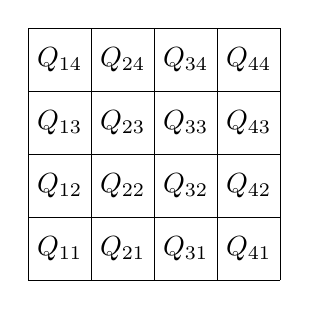
\begin{tikzpicture}[scale=0.8]
        \draw (0,0) grid (4,4);
        \foreach \x in {1,2,3,4}  {   
            \foreach \y in {1,2,3,4} {
                \node (A\x\y) at (\x-0.5,\y-0.5) {$Q_{\x\y}$};
            }
        }
    \end{tikzpicture}
        \]

            \begin{remark*}[teilweise mündlich]
                Genauer gesagt würden wir nach dem Lebesgue-Lemma ein $\delta$ erhalten, sodass jede offene Menge mit  $\diam < \delta$ in einem der $U_i$ liegt. Aber natürlich können wir dann  $m$ groß genug machen, sodass ein abgeschlossenes Quadrat in einer etwas größeren offenen Menge liegt, die Durchmesser  $<\delta$ hat.
            \end{remark*}
            Wir wollen im Folgenden eine Familie von stetigen Abbildungen $\tilde{H}_{ij}\colon  Q_{ij}\to E$ konstruieren, die $H$ lokal, d.h. auf  $Q_{ij}$, heben und untereinander 'kompatibel' sind, genauer:
            \begin{enumerate}[i)]
                \item $ p \circ  \tilde{H}_{ij} = H|_{Q_{ij}}$ ($\tilde{H}_{ij}$ ist Hebung auf $Q_{ij}$)
                \item $\tilde{H}_{11}(0,0) = \tilde{w}_0(0) = \tilde{w}_1(0)$ ($\tilde{H}_{11}$ hebt $w_0(0)$ auf $\tilde{w}_0(0)$)
                \item $(\tilde{H}_{ij})|_{Q_{ij} \cap  Q_{i'j'}} = (\tilde{H}_{i'j'})|_{Q_{/j} \cap  Q_{i'j'}}$ (die lokalen Hebungen sind auf ihren Schnittmengen, d.h. den Rändern der Quadrate, identisch)
            \end{enumerate}

            Dies führen wir rekursiv in der Reihenfolge $11, 12, \ldots, 1m$, $21, 22, \ldots, 2m$, $\ldots, 3m, \ldots, mm$ durch, wobei wir in jedem Schritt obige Bedingungen sicherstellen, d.h. wir beweisen diese Aussagen parallel mittels Induktion.

            Seien also $1\leq i,j\leq m$ gegeben, sodass wir die vorherigen $\tilde{H}_{ij}$ bereits definiert haben. Wir finden ein $k$, sodass $H(Q_{ij})$ in $U_k$ liegt, über dem die Überlagerung trivial ist, also können wir eine lokale Umkehrfunktion  $s\colon  U \to  E$ wählen, die zusätzlich den Startpunkt
    \begin{equation}
        \label{eq:def-von-s}
        s\left(H\left( \frac{i-1}{m}, \frac{j-1}{m} \right) \right) = \begin{cases}
            \tilde{w}_0(0) & i=j=1 \\
            \tilde{H}_{i-1,j}\left( \frac{i-1}{m}, \frac{j-1}{m} \right) & i>1 \\
            \tilde{H}_{i,j-1}\left( \frac{i-1}{m}, \frac{j-1}{m} \right) & j>1
        \end{cases}
    \end{equation}
    besitzt, d.h. $s$ hebt die 'linke untere Ecke' von  $H(Q_{ij})$ auf den gleichen Punkt wie eine der vorherigen Abbildungen $\tilde{H}_{i',j'}$ (bzw. auf den Anfangspunkt $\tilde{w}_0(0)$, wenn wir die erste Abbildung definieren), damit die Abbildungen letztendlich zusammenpassen.
    \begin{remark}
        Da $\tilde{H}_{i-1,j}$ und $ \tilde{H}_{i,j-1}$ auf der Ecke $\left( \frac{i-1}{m}, \frac{j-1}{m} \right) $ übereinstimmen, ist das wohldefiniert für $i,j > 1$. Dazu ist insbesondere wichtig, dass wir Eigenschaft iii) für $i-1,j$ und  $i,j-1$ bereits induktiv annehmen können.
    \end{remark}

    Mit dieser Umkehrabbildung setzen wir nun naheliegenderweise $\tilde{H}_{ij}\coloneqq  s \circ  H|_{Q_{ij}}$. Wir müssen nun die Eigenschaften i) - iii) prüfen. i) ergibt sich unmittelbar aus der Wahl von $s$ mittels
    \[
        p \circ  \tilde{H}_{ij} \stackrel{\text{def}}{=} p \circ  (s \circ  H|_{Q_{ij}}) = (p \circ  s) \circ  H|_{Q_{ij}} = \id_{U_k} \circ  H|_{Q_{ij}} =  H|_{Q_{ij}}
    .\] 

    Eigenschaft ii) ergibt sich unmittelbar aus der Definition in \autoref{eq:def-von-s}, Eigenschaft iii) müssen wir nur für das neu hinzugekommene $\tilde{H}_{ij}$ zeigen, und auch nur für den Schnitt mit den (potenziell) benachbarten Quadraten links und unter $Q_{ij}$, weil die Schnitte sonst leer sind. Also bleibt zu zeigen:

    \begin{claim}[linker Rand von $Q_{ij}$]
        Ist $i>1$, so ist  $\tilde{H}_{ij}|_{Q_{ij} \cap  Q_{i-1,j}} = \tilde{H}_{i-1,j} |_{Q_{ij} \cap Q_{i-1,j}}$.
    \end{claim}

    \begin{subproof}
        Es ist $Q_{ij}\cap Q_{i-1,j} = \left \{\frac{i-1}{m}\right\} \times [\frac{j-1}{m},\frac{j}{m}]$ und kann somit durch
        \[
            t \mapsto \left( \frac{i-1}{m}, \frac{j-1 + t}{m} \right) 
        .\] 
        für $t\in [0,1]$ parametrisiert werden.

        Die entsprechenden Wege
        \begin{IEEEeqnarray*}{rCl}
            t &\mapsto &\tilde{H}_{ij}\left( \frac{i-1}{m}, \frac{j-1+t}{m} \right)  \\
            t & \mapsto & \tilde{H}_{i-1,j} \left( \frac{i-1}{m}, \frac{j-1+t}{m} \right) 
        \end{IEEEeqnarray*}
        heben alse den Weg $t \mapsto H\left( \frac{i-1+t}{m}, \frac{j-1+t}{m} \right) $ und stimmen für $t=0$ am Wert
        \[
            \tilde{H}_{ij}\left( \frac{i-1}{m}, \frac{j-1}{m} \right) \stackrel{\text{def}}{=} \tilde{H}_{i-1,j}\left( \frac{i-1}{m},\frac{j-1}{m} \right)  
        .\] überein (vergleiche auch wieder \autoref{eq:def-von-s}). Nach dem \nameref{thm:weghebungssatz} sind also beide Wege gleich, also stimmen $\tilde{H}_{ij}, \tilde{H}_{i-1,j}$ entsprechend überein.
\end{subproof}
\begin{claim}[unterer Rand von $Q_{ij}$]
    Ist $j>1$, so ist  $\tilde{H}_{ij}|_{Q_{ij}\cap Q_{i,j-1}} = \tilde{H}_{i,j-1}|_{Q_{ij}\cap Q_{i,j-1}}$
\end{claim}
\begin{subproof}
    Völlig analog zu Behauptung 1, der Schnitt ist der untere Rand von $Q_{ij}$ und kann analog parametrisiert werden.
\end{subproof}

Damit haben wir zusammen eine Abbildung $\tilde{H}_{ij}$ mit den geforderten Eigenschaften i) - iii) konstruiert. Es ist nun leicht zu prüfen, dass wir die $\tilde{H}_{ij}$ zu einer Abbildung
    \begin{equation*}
    \tilde{H}: \left| \begin{array}{c c l} 
    I^2 & \longrightarrow & E \\
    (x,y) & \longmapsto &  \tilde{H}_{ij}(x,y) \text{, wobei $i,j$ so, dass  $(x,y)\in Q_{ij}$} 
    \end{array} \right.
\end{equation*}
zusammenfügen können, die die geforderten Eigenschaften besitzt.


\item[Eindeutigkeit] Sei $\tilde{\tilde{H}}$ eine weitere Hebung mit $\tilde{\tilde{H}} (0,0) = \tilde{w}_0(0)$. Sei $(t,s) \in I^2$ und $w$ ein Weg von  $(0,0)$ nach  $(t,s)$ in  $I^2$ (z.B. der lineare Weg). Dann sind $\tilde{H} \circ w$ und $\tilde{\tilde{H}} \circ  w$ Hebungen von $H\circ  w$. mit demselben Anfangspunkt. 

    Nach der Eindeutigkeit im \nameref{thm:weghebungssatz} sind also auch schon $\tilde{H} \circ w$ und $\tilde{\tilde{H}} \circ w$ gleich, insbosender stimmen sie an $(t,s)$ überein, und somit  $\tilde{\tilde{H}}(t,s) = \tilde{H}(t,s) $. Da $(t,s)\in I^2$ beliebig war, folgt also wie gewünscht $\tilde{H} = \tilde{\tilde{H}} $.
\end{description}
\begin{enumerate}[i)]
    \setItemnumber{2}
\item Der Weg $\tilde{H}(-,0)$ hebt $H(-,0)= w_0$ mit Anfangspunkt $\tilde{w}_0(0)$. Auch $\tilde{w}_0$ ist ein solcher Lift. Aus der Eindeutigkeit im \nameref{thm:weghebungssatz} folgt also genau $\tilde{H}(-,0) = \tilde{w}_0$. $\tilde{H}(-,0)$ ist in folgender Skizze blau markiert. Bevor wir jedoch etwas über $\tilde{H}(-,1)$ aussagen können, müssen wir erst noch über die linke Kante von $I^2$ etwas lernen (im Bild orange).

    \begin{minipage}{\textwidth}
        \centering
    \incfig{verschiedene-weghebungen-bei-homotopiehebung}
    \end{minipage}

    Weiter hebt $\tilde{H}(0,-)$ den Weg $H(0,-) = c_{w_0(0)}$, weil $H$ eine Homotopie relativ Anfangspunkt ist. Auch  $c_{\tilde{w}_0(0)}$ ist eine solche Hebung (mit gleichem Anfangspunkt), also ist bereits $\tilde{H}(0,-) = c_{\tilde{w}_0(0)}$.

    Damit folgt bereits, dass $\tilde{H}$ eine Homotopie relativ Anfangspunkt ist, und dass $\tilde{H}(0,1) = c_{\tilde{w}_0(0)}$. Also hebt der Weg $\tilde{H}(-,1)$ den Weg $H(-,1) = w_1$ \textit{mit Anfangspunkt} $\tilde{w}_0(0) = \tilde{w}_1(0)$, und wegen der Eindeutigkeit der Wegeliftung erhalten wir wie gewünscht $\tilde{H}(-,1) = \tilde{w}_1$.
\item Der Weg $\tilde{H}(1,-)$ hebt nun $H(1,-)$. Ist  $H(1,-)$ konstant, dann auch  $\tilde{H}(1,-)$, weil wir auch die konstante Hebung haben, und die Hebung eindeutig ist.
\end{enumerate}
\end{proof}
\section{Beispiele für $\pi_1$}

\begin{definition}
    Ein topologischer Raum $X$ heißt  \vocab[Topologischer Raum!einfach zusammenhängend]{einfach zusammenhängend}, falls $X$ wegzusammenhängend ist und je zwei Wege mit gleichen Anfangs- und Endpunkten homotop sind (relativ Anfangs- und Endpunkt).

\begin{minipage}{\textwidth}
    \centering
    \incfig{einfach-zusammenhaengender-raum}
\end{minipage}
\end{definition}

\begin{lemma}
    Ein Raum $X$ ist einfach zusammenhängend genau dann, wenn er wegzusammenhängend ist und  $\pi_1(X,x)$ trivial ist für ein (oder äquivalent alle) $x\in X$.
\end{lemma}

\begin{proof}
'$\implies$' Spezialfall der Definition.    

'$\impliedby$' Seien $w, w'\colon I \to X$ Wege mit $w(0) = w'(0) =x$ und  $w(1) = w'(1) = y$. Dann ist 
 \[
     w \simeq (w' \star  \overline{w'}) \star w \simeq w' \star (\overline{w'} \star w) \stackrel{\pi_1(X,y) = 0}{\simeq} w'
.\] 
\end{proof}

